\documentclass{article}

\usepackage{tikz}
\usetikzlibrary{graphs.standard, quotes}
\usepackage{amsthm}
\usepackage{enumitem}

\title{CSCI 570 - Fall 2021 - HW 8}
\author{Shangning Xu}

\begin{document}

\maketitle

\section*{Graded}

\begin{enumerate}
    \item
    \begin{enumerate}
        \item Refer to Figure~\ref{fig:1a}.
        \begin{figure}[ht]
            \centering
            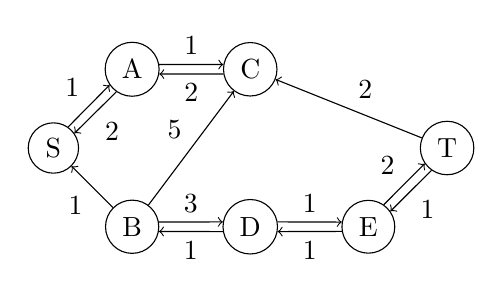
\begin{tikzpicture}
                \foreach \position / \label in {(0, 1)/S, (1, 2)/A, (1, 0)/B, (2.5, 2)/C, (2.5, 0)/D, (4, 0)/E, (5, 1)/T}
                    \node (\label) at \position [circle, draw] {\label};
                
                \draw [->] (node cs: name=S, angle=55) -- node [above left] {1} (node cs: name=A, angle=-145);
                \draw [->] (node cs: name=A, angle=-125) -- node [below right] {2} (node cs: name=S, angle=35);
                
                \draw [->] (B) -- node [below left] {1} (S);
            
                \draw [->] (node cs: name=A, angle=10) -- node [above] {1} (node cs: name=C, angle=170);
                \draw [->] (node cs: name=C, angle=-170) -- node [below] {2} (node cs: name=A, angle=-10);
            
                \draw [->] (node cs: name=B, angle=10) -- node [above] {3} (node cs: name=D, angle=170);
                \draw [->] (node cs: name=D, angle=-170) -- node [below] {1} (node cs: name=B, angle=-10);
            
                \draw [->] (B) -- node [above left] {5} (C);
            
                \draw [->] (node cs: name=D, angle=10) -- node [above] {1} (node cs: name=E, angle=170);
                \draw [->] (node cs: name=E, angle=-170) -- node [below] {1} (node cs: name=D, angle=-10);
            
                \draw [->] (node cs: name=E, angle=55) -- node [above left] {2} (node cs: name=T, angle=-145);
                \draw [->] (node cs: name=T, angle=-125) -- node [below right] {1} (node cs: name=E, angle=35);
            
                \draw [->] (T) -- node [above right] {2} (C);
            \end{tikzpicture}
            \caption{Residual graph for Question 1 (a)}
            \label{fig:1a}
        \end{figure}
        
        \item The max-flow value is 3. The minimum cut is $(\{S, A, C\}, \{B, D, E, T\})$.
    \end{enumerate}

    \item
    \begin{enumerate}
        \item We define the corresponding flow network to an instance of the given problem as follows:
        \begin{enumerate}
            \item One vertex for each student and class, with an additional source and sink vertices.
            \item Add an edge between each student and the source with capacity $m$.
            \item Add an edge between each class $c_j$ and the sink with capacity $q_j$.
            \item Add an edge between each student $s_j$ and classes they want to sign up for with unit capacity.
        \end{enumerate}

        Our algorithm runs the Ford-Fulkerson method over the flow network to obtain a maximum flow. If the maximum flow value is exactly $mn$, then all students can be enrolled as full-time students.

        The algorithm is correct because for each integer-valued flow, we can intuitively construct an assignment of students to classes so that the flow between the source and $s_j$ is the number of classes they can sign up for within class capacity. When the maximum flow value is $mn$, each source-to-student edge must have flow $m$, meaning that it is possible for every student to be enrolled in $m$ classes.
        
        \item We tweak the flow network in (a) by removing edges between students and classes when the student is not enrolled in the class, change capacity of edges between source and students to $r$ and capacity of edges between classes and sink to 1. We solve for the maximum flow value on the new flow network. If the flow value is exactly the number of classes, then the required selection exists.
        
        The algorithm is correct because given an integer-valued flow, we construct a selection of student representative by assigning a student to a class if there is flow between the corresponding edge. When the flow value is exactly the number of classes, it means that every class has a representative and no student is a representative to more than $r$ classes.
    \end{enumerate}

    \item
    \begin{enumerate}
        \item False. Consider the following flow network. After replacing the edges, the edge $(s, t)$ is added, allowing a maximum flow with value 100.
        \begin{center}
            \tikz \graph [math nodes] {
                subgraph I_n [V={v, t, s}, clockwise, nodes={draw, circle}];
                s -> ["1"] v -> ["1"] t -> ["100"] s;
            };
        \end{center}

        \item True. By definition, there is at most one $D$-scaling phase for any $D$ in the capacity-scaling algorithm, so an edge $e$ can be present in $G_f(D)$ in at most one $D$-scaling phase.
    
        \item True.
        \begin{proof}
            After all edges are multiplied by $k$, for any cut $(S, T)$ of the flow network, its new capacity
            \[
                c'(S, T) = \sum_{u \in S} \sum_{v \in T} kc(u, v) = k \sum_{u \in S} \sum_{v \in T} c(u, v) = kc(S, T).
            \]

            Because cut capacities are all positive, after multiplied by $k$, the original minimum cut's capacity remains minimum among all cuts.
        \end{proof}

        \item False. Consider the following flow network. After increasing edge capacities, the maximum flow increases from 2 to $4 > 3$.
        \begin{center}
            \tikz \graph [math nodes, edge label=1] {
                subgraph I_n [V={v, t, s}, clockwise, nodes={draw, circle}];
                s -> v -> t;
                s -> t;
            };
        \end{center}
    \end{enumerate}

    \item We can repeatedly run the Ford-Fulkerson method on the flow network to find the maximum flow, delete any edge from the corresponding minimum cut and find a new maximum flow, until $k$ edges are deleted from the graph.
    
    When the edges don't have unit capacities, we can delete the edge with maximum capacity that crosses the minimum cut during each iteration.
\end{enumerate}

\section*{Ungraded}

\begin{enumerate}[resume]
    \item We define the corresponding flow network to an instance of the given problem as follows:
    \begin{enumerate}
        \item Add a vertex for every tourist and every currency, along with a source and sink.
        \item Add an edge between the source and each tourist $t_k$ with capacity $F_k$, an edge between each currency $c_j$ and the sink with capacity $B_j$ and an edge between $t_k$ and $c_j$ with capacity $S_{kj}$.
    \end{enumerate}

    We run the Ford-Fulkerson method on the flow network to obtain a maximum flow. If the maximum flow value is exactly $\sum_{k = 1}^n F_k$, then all tourists' requests can be fulfilled.

    \item We define the corresponding flow network to an instance of the given problem as follows:
    \begin{enumerate}
        \item Add a source and connect it to each entrance. Add a sink and connect each exit to it.
        \item Split each vertex $v$ that is neither an entrance nor an exit into two vertices $v_\textrm{in}$ and $v_\textrm{out}$ with edge $(v_\textrm{in}, v_\textrm{out})$. Connect $v$'s incoming edges to $v_\textrm{in}$ and outgoing edges to $v_\textrm{out}$.
        \item Assign unit capacity to each edge.
    \end{enumerate}

    We run the Ford-Fulkerson method on the flow network to obtain a maximum flow. If the maximum flow value is exactly $k$, then there exists an arrangement for the private showings where no client will see each other.

    \item The minimum vertex cover for a bipartite graph is the smallest vertex set between the two vertex sets that partition the graph. Therefore, our algorithm first partitions the graph into two disjoint vertex sets and compare the size of the smaller set to $k$. The graph has a vertex cover of at most size $k$ if and only if the size of the smaller set is less than $k$.
    
    To partition the graph and compute the size of both sets, we run BFS from any vertex and note that levels in the BFS tree alternate between the two sets in the bipartite graph. Therefore, we only need to count the number of vertices in alternating levels to compute the set size.
\end{enumerate}

\end{document}
